
\begin{frame}
	\begin{block}{CERN}
		At CERN -- European Organization for Nuclear Research -- scientists are probing the fundamental structure of the universe. Using the world's largest and most powerful particle accelerators as well the most complex and precise detectors, physicists study the fundamental particles and their interactions.
	\end{block}
	\begin{block}{Accelerator Complex and LHC}
		The accelerator complex at CERN is a succession of machines that accelerate beams of particles to increasingly higher energies, before injecting them into the next machine.
		
		The Large Hadron Collider (LHC) is the last machine in this chain and can accelerate particle beams up to a record energy of 6.5 TeV. The beams are then transferred into two oppositely circulating beam pipes and finally collide inside four detectors -- ALICE, ATLAS, CMS and LHCb.
	\end{block}
\end{frame}


\begin{frame}
	\begin{textblock}{2}(1,0)
		\begin{figure}
			
\includegraphics[width=\textwidth]{figures/BLonD_logo_header}
		\end{figure}
	\end{textblock}
	\begin{textblock}{2}(3,0)
		\begin{figure}
			
\includegraphics[width=\textwidth]{figures/python-logo}
		\end{figure}
	\end{textblock}
	\begin{textblock}{2}(5,0)
	\begin{figure}
		
\includegraphics[width=\textwidth]{figures/cpp-logo}
	\end{figure}
	\end{textblock}
	\vspace{1.5cm}
	\begin{block}{}
		The \underline{B}eam \underline{Lon}gitudinal \underline{D}ynamics simulator \footnote{http://blond.web.cerh.ch}  is a unique code developed at CERN to model beam motion in synchrotrons. Important upgrades of beam parameters are based on BLonD simulations. The code is modular and each simulation is composed of a pipeline of different physics modules. It is written in Python with C/C++ extensions for the computational kernels.
		
		BLonD is an open-source project \footnote{https://github.com/blond-admin/BLonD} with more than 10 contributors and numerous users. Some of the most important conclusions drawn using BLonD can be found in the literature \footfullcite{timko2015studies} \footfullcite{timko2016benchmarking} \footfullcite{lasheen2015synchrotron}.
	\end{block}
\end{frame}

\begin{frame}
%		\begin{columns}[t]
		\begin{textblock}{8.8}(0.,0)
			\begin{figure}[h]
%				\hspace{-12pt}
				\animategraphics[loop, autoplay, width=\textwidth] {8} {figures/LHC_Blow-up/LHC_Blow-up-}{0}{89} %89
%				\caption*{Insert caption}
			\end{figure}
		\end{textblock}
		\begin{textblock}{7.2}(8.8,0)
			\begin{block}{LHC controlled longitudinal emittance Blow-Up}
				An RF noise injection targeting the bunch core maintains a constant stability threshold by increasing the emittance as the sqrt of energy.	
%In the LHC, maintaining a constant stability threshold requires an increase of the longitudinal emittance as the square-root of energy. This is done by RF phase noise injection that targets the bunch core. 
%				The noise can either be injected through the phase loop or directly through the cavity; in both cases, 
				A feedback on the noise amplitude keeps constant FWHM bunch length.
%				Simulations reveal that the bunch core becomes rounder during the process, while the tail population remains inside a certain area.
			\end{block}
		\end{textblock}
		\begin{textblock}{4.8}(0.0,7)
			\begin{figure}[h]
				\animategraphics[loop, autoplay, width=\textwidth] {6} {figures/PS-SPS_Transfer/PS-SPS_Transfer-}{0}{104} %104
%				\caption*{Insert caption}
			\end{figure}
		\end{textblock}
		\begin{textblock}{11.2}(4.8,7.5)
			\begin{block}{PS-to-SPS Transfer}
				In the PS, the LHC-type 25ns beam is created through RF manipulations. After the injection of 4+2 bunches from the PSB, a triple splitting is performed and the bunches are accelerated. At flat top, each bunch is twice split in two, resulting in 72 bunches. Finally, an adiabatic bunch shortening and a bunch rotation provide bunches that are short enough to be injected into the 200 MHz buckets of the SPS.
			\end{block}
		\end{textblock}

%		\end{columns}
\end{frame}


\begin{frame}
%	\begin{textblock}{15}(0.5,3)
	\begin{block}{BLonD++}
	BLonD++ \footnote{https://github.com/blond-admin/BLonD-cpp} is the C++ version of BLonD. It features openMP multi-threading and auto-vectorization friendly computational kernels. BLonD++ has been proved to perform particularly faster than BLonD on time-consuming, complex simulations.
	\end{block}

%	\end{textblock}
%	\begin{textblock}{6}(0,7)
	\begin{block}{}
	
	\begin{columns}[t]
		\column[t]{0.52\textwidth}
		\vspace{-1.4cm}
		\begin{figure}
			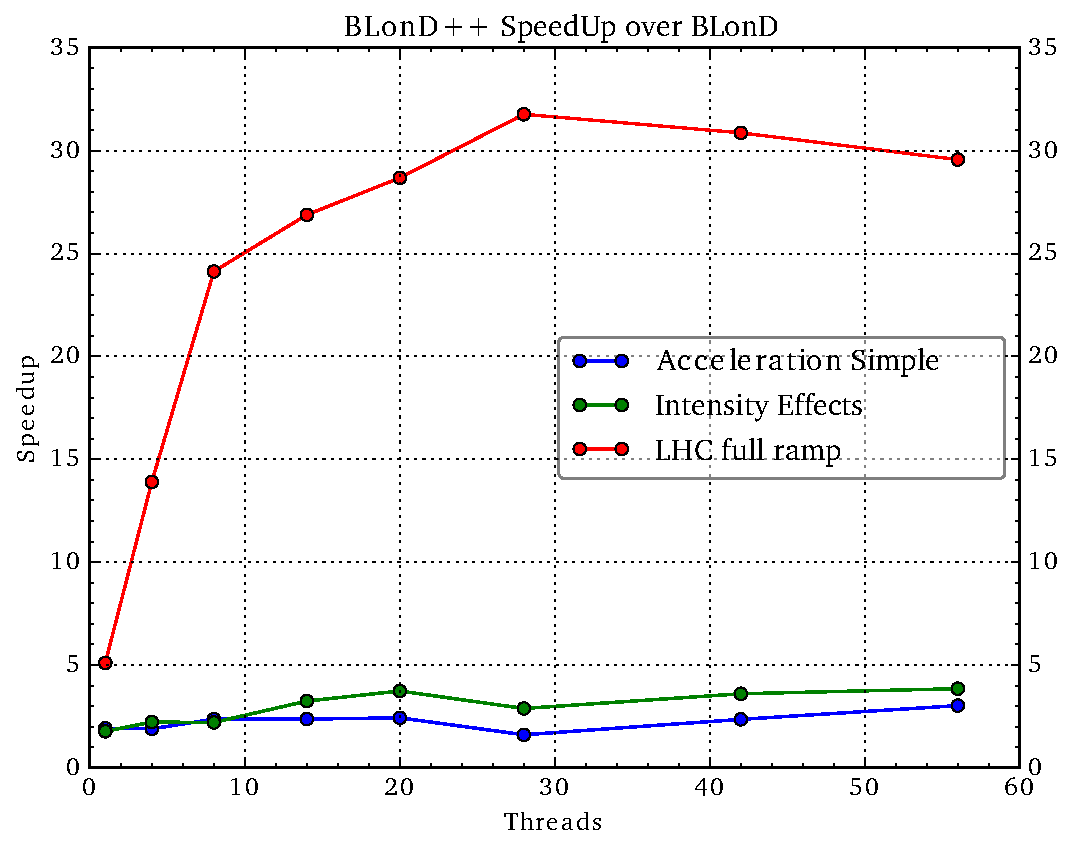
\includegraphics[width=\textwidth]{figures/BLonDpp-speedup2}
		\end{figure}
		
		\column[t]{0.5\textwidth}
%		\vspace{-0.5cm}
		Each line corresponds to a test-case of different complexity level. The top Speed-Up achieved in the two less complex test-cases is up to 3.0X and 3.9X respectively. However, the results are different in the most complex case, demonstrating a maximum Speed-Up of 31.8X. 
	\end{columns}
	\end{block}
%	\end{textblock}
\end{frame}

\begin{frame}
%	\frametitle{Motivation}
	\begin{block}{Motivation}
		The present CERN computing infrastructure is composed of heterogeneous general purpose CPUs. The complexity of physics problems that can be modelled is restricted due to runtime limitations. A dedicated computer architecture is necessary to meet the continuously growing computational needs of the longitudinal beam dynamics field.
	\end{block}

	\begin{block}{Ongoing Work}
		Existing high-performance CERN infrastructure and software methods are being explored for their suitability to address performance and scalability issues of BLonD simulations. The interaction between different modules is investigated in detail.
	\end{block}

	\begin{block}{Future Studies}
		Eventually, combinations of CPUs and accelerators, including Xeon Phis, GPUs and FPGAs,  will be evaluated. Ideally, the outcome of the thesis will be a concrete proposal for an HPC system to serve the longitudinal beam dynamics studies. 
	\end{block}
\end{frame}



